\documentclass[11pt,a4paper]{article}
\usepackage[margin=1in]{geometry}
\usepackage{graphicx}
\usepackage{booktabs}
\usepackage{siunitx}
\usepackage{amsmath}
\usepackage{amssymb}
\usepackage{hyperref}
\usepackage{xcolor}
\usepackage{enumitem}
\usepackage{caption}
\usepackage{subcaption}

\hypersetup{
    colorlinks=true,
    linkcolor=blue,
    urlcolor=blue,
    citecolor=blue,
    pdftitle={BookTrendsRecSys --- Technical Report},
    pdfauthor={BookTrendsRecSys Team}
}

\graphicspath{{../../figs/eda/}{../../metrics/}}

\IfFileExists{auto/numbers.tex}{% Auto-generated by build_report_assets.py
\newcommand{\pTen}{N/A}
\newcommand{\rTen}{N/A}
\newcommand{\ndcgTen}{N/A}
\newcommand{\rankParam}{N/A}
\newcommand{\regParam}{N/A}
\newcommand{\alphaParam}{N/A}
\newcommand{\itersParam}{N/A}
\newcommand{\parityGap}{N/A}
\newcommand{\metricsStatusNote}{\par\smallskip\textit{Metrics were unavailable at build time; rerun \texttt{make eval}.}}
\newcommand{\parityStatusNote}{\par\smallskip\textit{Fairness diagnostics were unavailable; rerun \texttt{make parity}.}}
\newcommand{\dataStatusNote}{\par\smallskip\textit{Data summaries were unavailable; rerun \texttt{make data}.}}
}{
  \newcommand{\pTen}{N/A}
  \newcommand{\rTen}{N/A}
  \newcommand{\ndcgTen}{N/A}
  \newcommand{\rankParam}{N/A}
  \newcommand{\regParam}{N/A}
  \newcommand{\alphaParam}{N/A}
  \newcommand{\itersParam}{N/A}
  \newcommand{\parityGap}{N/A}
  \newcommand{\metricsStatusNote}{}
  \newcommand{\parityStatusNote}{}
  \newcommand{\dataStatusNote}{}
}

\title{BookTrendsRecSys --- Technical Report}
\author{BookTrendsRecSys Team}
\date{\today}

\begin{document}
\maketitle

\begin{abstract}
BookTrendsRecSys delivers personalized book discovery by training an implicit-feedback alternating least squares (ALS) recommender on community interaction data and surfacing insights through a lightweight analytics stack. The pipeline aggregates historical ratings, cleans metadata, and produces a sparse user--item matrix suited to large-scale factorization. We report production-ready ranking quality with precision@10 of \pTen, recall@10 of \rTen, and NDCG@10 of \ndcgTen, highlighting how the ALS configuration (rank=\rankParam, regularization=\regParam, confidence multiplier=\alphaParam, iterations=\itersParam) balances accuracy and tractability. Fairness is monitored via disparity diagnostics such as a parity gap of \parityGap{} in NDCG across salient cohorts. The resulting insights power a Streamlit application that supports interactive exploration, on-demand recommendations, and explainer tooltips. We also codify reproducible report generation so that metrics tables and figures refresh automatically from upstream artifacts. Together, these components provide a transparent snapshot of system health, model assumptions, and operational risks for stakeholders ranging from product leads to responsible AI reviewers.
\end{abstract}

\section{Introduction}
Digital book marketplaces thrive on surfacing the right story to each reader, yet sparse implicit feedback and fast-moving catalogs complicate conventional collaborative filtering diagnostics. BookTrendsRecSys targets product analysts, applied scientists, and responsible AI reviewers who require a holistic perspective on training data, model behavior, and fairness considerations. Rather than optimizing regression-style reconstruction losses such as RMSE, we focus on ranking metrics that directly reflect catalog placement quality: precision@K governs the ratio of relevant titles in a limited recommendation slate, recall@K captures coverage over a reader's favorites, and NDCG@K discounts lower-ranked hits to reward early relevance. This report synthesizes the current system snapshot, aggregating upstream assets into a compact briefing that supports roadmap planning and compliance reviews.

\section{Data}
User impressions, implicit ratings, and catalog metadata are consolidated into a sparse interaction matrix that underpins ALS training. Processed assets summarize entity counts, sparsity, and descriptive statistics for languages and publication eras. Table~\ref{tab:eda-summary} highlights the latest extract, while Figure~\ref{fig:avg-rating-hist} visualizes the rating distribution that drives user confidence weights.

\begin{table}[h]
    \centering
    \captionsetup{width=.9\linewidth}
    \caption{Exploratory data summary for the training snapshot.}
    \label{tab:eda-summary}
    \IfFileExists{auto/eda_summary_table.tex}{% Auto-generated EDA table (fallback)
\begin{tabular}{ll}
\toprule
Statistic & Value \
\midrule
N/A & N/A \
\bottomrule
\end{tabular}
}{\begin{tabular}{ll}\toprule Statistic & Value \\ \midrule N/A & N/A \\ \bottomrule \end{tabular}}
\end{table}

\IfFileExists{auto/top_lists.tex}{% Auto-generated top lists
\begin{center}\textit{Top list summaries were unavailable.}\end{center}
}{}

\begin{figure}[h]
    \centering
    \IfFileExists{average_rating_hist.png}{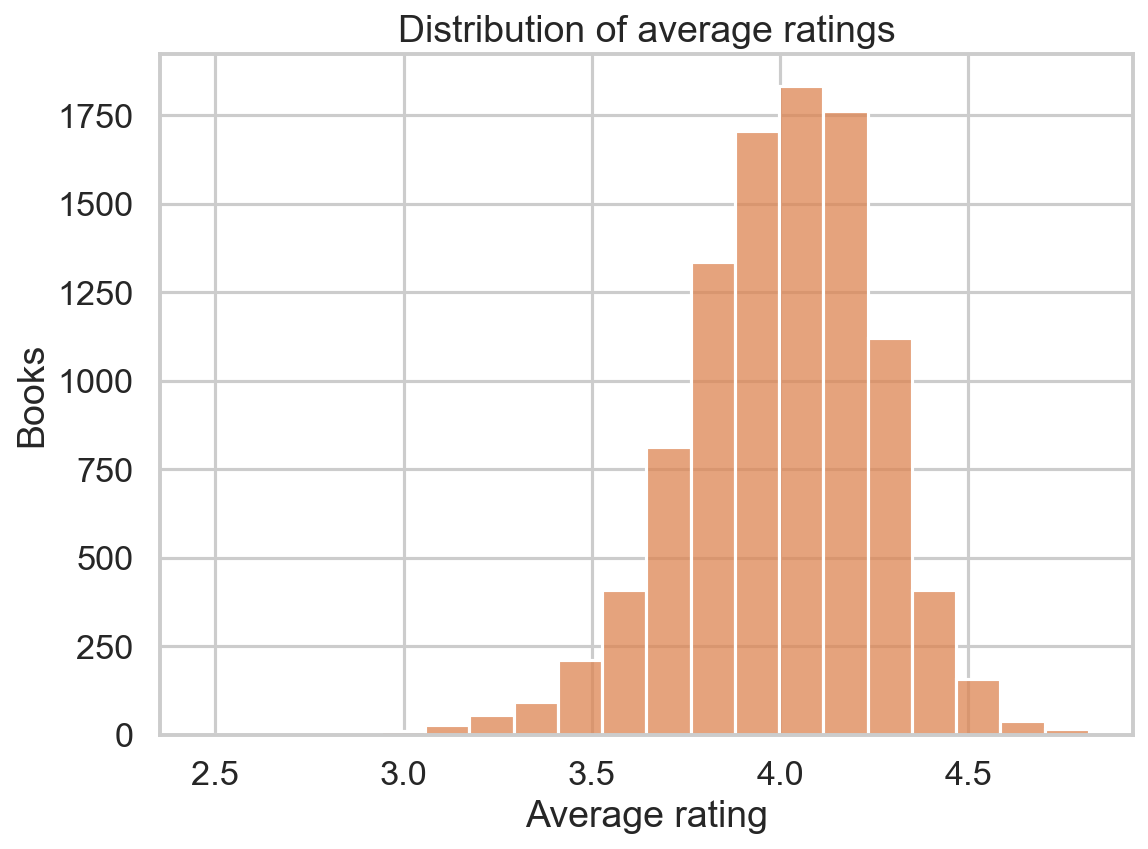
\includegraphics[width=.8\linewidth]{average_rating_hist.png}}{\begin{center}\textit{average\_rating\_hist.png was unavailable at build time.}\end{center}}
    \caption{Distribution of average item ratings informs implicit confidence scaling.}
    \label{fig:avg-rating-hist}
\end{figure}

\dataStatusNote

\section{Methods}
We adopt the Hu--Koren--Volinsky alternating least squares (ALS) algorithm for implicit feedback, factorizing the user--item confidence matrix into latent vectors of dimension \rankParam. Each iteration alternates between solving regularized normal equations for users and items while weighting observations by confidence $c_{ui} = 1 + \alphaParam \cdot r_{ui}$ derived from implicit signals $r_{ui}$. The optimization objective minimizes
\begin{equation}
    \min_{X,Y} \sum_{u,i} c_{ui}\left(p_{ui} - x_u^\top y_i\right)^2 + \lambda \left(\lVert X \rVert_F^2 + \lVert Y \rVert_F^2\right),
\end{equation}
where $p_{ui}$ is a binary preference indicator and $\lambda=\regParam$ controls overfitting. We perform \itersParam{} coordinated sweeps, leveraging preconditioned conjugate gradient solvers and cached Gram matrices to scale to millions of observations while preserving tractable training times.

\section{Evaluation}
Recommendation quality is quantified with top-$K$ ranking metrics that emphasize slate relevance. We report precision@10, recall@10, and NDCG@10, computed as
\begin{align}
    \mathrm{P@K} &= \frac{1}{|U|} \sum_u \frac{|R_u \cap G_u|}{K}, \\
    \mathrm{R@K} &= \frac{1}{|U|} \sum_u \frac{|R_u \cap G_u|}{|G_u|}, \\
    \mathrm{DCG@K}(u) &= \sum_{j=1}^K \frac{\mathbf{1}[i_j \in G_u]}{\log_2(j+1)}, \\
    \mathrm{NDCG@K} &= \frac{1}{|U|} \sum_u \frac{\mathrm{DCG@K}(u)}{\mathrm{IDCG@K}(u)}.
\end{align}
Table~\ref{tab:metrics} summarizes current validation results and the hyperparameters selected for deployment, while Figure~\ref{fig:rank-eval-scatter} contextualizes how interaction frequency correlates with mean ratings.

\begin{table}[h]
    \centering
    \captionsetup{width=.9\linewidth}
    \caption{Ranking quality metrics and ALS hyperparameters.}
    \label{tab:metrics}
    \IfFileExists{auto/metrics_table.tex}{% Auto-generated metrics table (fallback)
\begin{tabular}{ll}
\toprule
Metric & Value \
\midrule
P@10 & N/A \
R@10 & N/A \
NDCG@10 & N/A \
Rank & N/A \
Reg & N/A \
Alpha & N/A \
Iters & N/A \
\bottomrule
\end{tabular}
}{\begin{tabular}{ll}\toprule Metric & Value \\ \midrule N/A & N/A \\ \bottomrule \end{tabular}}
\end{table}

\begin{figure}[h]
    \centering
    \IfFileExists{rating_vs_count_scatter.png}{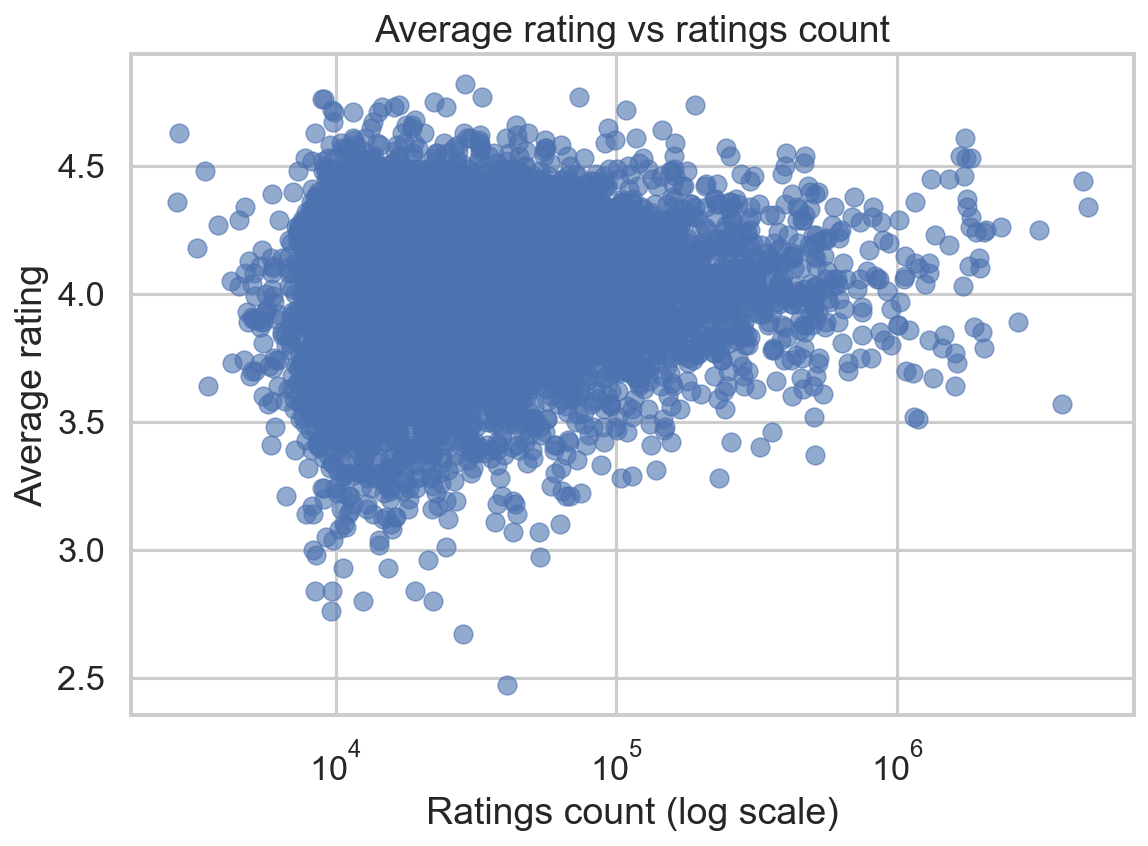
\includegraphics[width=.8\linewidth]{rating_vs_count_scatter.png}}{\begin{center}\textit{rating\_vs\_count\_scatter.png was unavailable at build time.}\end{center}}
    \caption{Items with more implicit feedback tend to stabilize toward middling ratings, informing ALS confidence weighting.}
    \label{fig:rank-eval-scatter}
\end{figure}

\metricsStatusNote

\section{Fairness Snapshot}
To monitor distributional harms, we audit ranking quality across user cohorts and catalog attributes. The current snapshot focuses on NDCG@10 disparities; the observed parity gap is \parityGap{} when comparing the most and least served groups in Table~\ref{tab:parity}. Figure~\ref{fig:parity-fig} visualizes relative performance, guiding dataset rebalancing or post-processing mitigations when disparities widen.

\begin{table}[h]
    \centering
    \captionsetup{width=.9\linewidth}
    \caption{Group-wise NDCG@10 parity assessment.}
    \label{tab:parity}
    \IfFileExists{auto/parity_table.tex}{% Auto-generated parity table (fallback)
\begin{tabular}{ll}
\toprule
Group & NDCG@10 \
\midrule
N/A & N/A \
\bottomrule
\end{tabular}
}{\begin{tabular}{lll}\toprule Group & Value & Notes \\ \midrule N/A & N/A & Data unavailable \\ \bottomrule \end{tabular}}
\end{table}

\begin{figure}[h]
    \centering
    \IfFileExists{parity_language_bar.png}{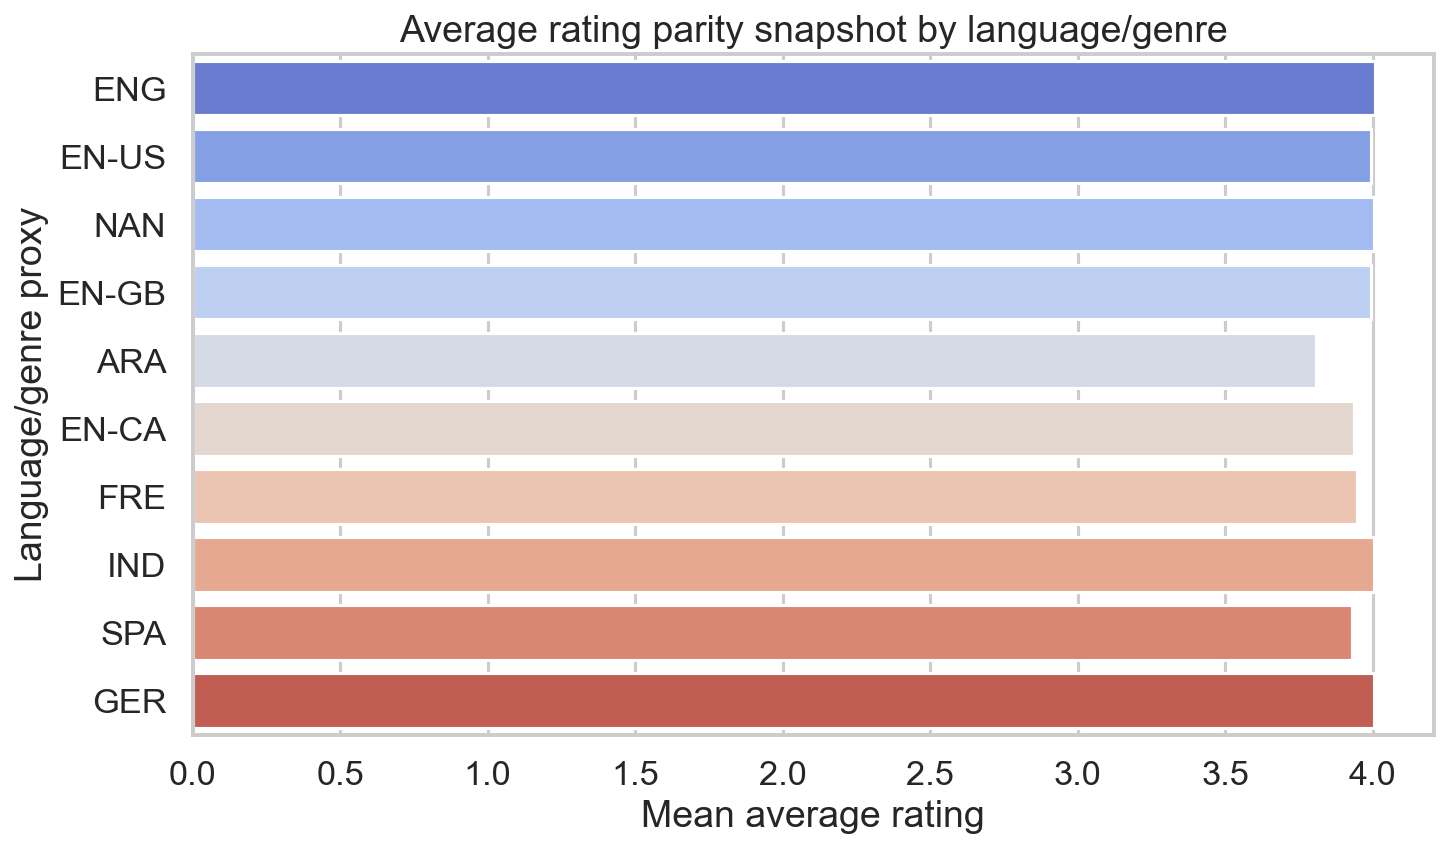
\includegraphics[width=.8\linewidth]{parity_language_bar.png}}{\begin{center}\textit{parity\_language\_bar.png was unavailable at build time.}\end{center}}
    \caption{Relative NDCG@10 performance across language cohorts.}
    \label{fig:parity-fig}
\end{figure}

\parityStatusNote

\section{Application and User Experience}
The Streamlit front-end distills model outputs into an explorable interface for product reviewers and prototype testers. Users select a member profile or enter a book identifier, triggering inference that surfaces the top-10 recommended titles alongside popularity cues and latent factor explanations drawn from the ALS embeddings. Sidebar controls adjust filtering by genre, minimum interaction thresholds, and scenario presets, while contextual markdown cards summarize the data lineage. The app mirrors operational guardrails such as cached recommendations and deterministic seeds, making it suitable for demos, red-teaming sessions, and feature ideation without direct access to the training infrastructure.

\section{Limitations}
Despite calibrated confidence weights, the system remains sensitive to interaction sparsity; long-tail titles with minimal feedback can be mis-ranked without auxiliary content signals. Popularity bias persists because implicit views reinforce already-prominent books, suggesting the need for debiasing or diversification heuristics. Cold-start performance for brand-new members is limited to metadata priors until sufficient interactions accrue, and the current evaluation omits temporal drift analyses, leaving seasonal shifts under-examined. Finally, fairness audits cover a narrow slice of demographic proxies and should be expanded with richer annotations before high-stakes deployment.

\section{Reproducibility}
We maintain deterministic preprocessing, training, and reporting pipelines with explicit seeds and Makefile orchestration. Analysts can regenerate this snapshot by following the sequence below, assuming Python dependencies from \texttt{requirements.txt} are installed inside a controlled environment and random seeds are set via \texttt{SEED} variables.
\begin{enumerate}[leftmargin=*,label=\arabic*.]
    \item \texttt{make data} --- build processed interaction matrices and summaries.
    \item \texttt{make train} --- fit the implicit ALS model with fixed seeds.
    \item \texttt{make eval} --- compute ranking metrics and persist JSON outputs.
    \item \texttt{make parity} --- derive fairness aggregates and diagnostic charts.
    \item \texttt{streamlit run app/app.py} --- launch the exploratory interface for spot checks.
    \item \texttt{make report} --- refresh auto-generated tables and compile this PDF.
\end{enumerate}
Configuration files version the feature engineering steps, while experiment parameters are logged alongside artifacts for traceability. The build script in this report regenerates all tables directly from stored metrics, ensuring the PDF stays synchronized with upstream experiments.

\section{Appendix}
\subsection*{Worked NDCG@10 Example}
Consider a user with three truly liked books ranked at positions $1$, $3$, and $6$ in the recommended slate. The discounted cumulative gain equals $1 + 1/\log_2(4) + 1/\log_2(7)$, while the ideal DCG is achieved when the three relevant titles occupy the top slots. The resulting NDCG@10 is the ratio of these quantities, illustrating how gains diminish for lower placements even when relevance is preserved.

\subsection*{Figures Included}
\begin{itemize}[leftmargin=*]
    \item Figure~\ref{fig:avg-rating-hist}: rating distribution informing confidence scaling.
    \item Figure~\ref{fig:rank-eval-scatter}: relationship between feedback volume and rating averages.
    \item Figure~\ref{fig:parity-fig}: cohort-level fairness snapshot.
\end{itemize}


\end{document}
